

% Gradient Info
  
\tikzset {_6ptlm6g7t/.code = {\pgfsetadditionalshadetransform{ \pgftransformshift{\pgfpoint{0 bp } { 0 bp }  }  \pgftransformscale{1 }  }}}
\pgfdeclareradialshading{_y5vaxgag9}{\pgfpoint{0bp}{0bp}}{rgb(0bp)=(0.29,0.56,0.89);
rgb(0bp)=(0.29,0.56,0.89);
rgb(0bp)=(0.29,0.56,0.89);
rgb(25bp)=(1,1,1);
rgb(400bp)=(1,1,1)}

% Gradient Info
  
\tikzset {_f8ci9uoe5/.code = {\pgfsetadditionalshadetransform{ \pgftransformshift{\pgfpoint{0 bp } { 0 bp }  }  \pgftransformscale{1 }  }}}
\pgfdeclareradialshading{_jj9izx5r0}{\pgfpoint{0bp}{0bp}}{rgb(0bp)=(0.82,0.01,0.11);
rgb(0bp)=(0.82,0.01,0.11);
rgb(21.33928571428571bp)=(1,1,1);
rgb(400bp)=(1,1,1)}
\tikzset{every picture/.style={line width=0.75pt}} %set default line width to 0.75pt        

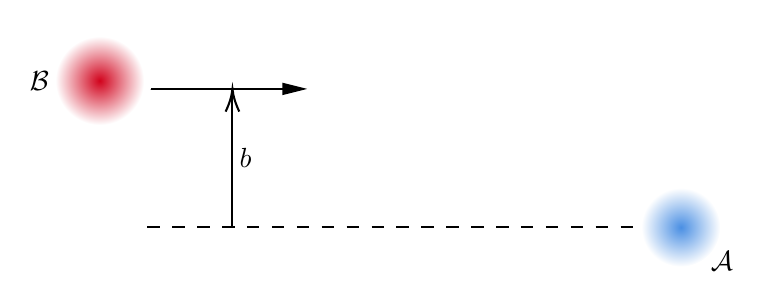
\begin{tikzpicture}[x=0.75pt,y=0.75pt,yscale=-1,xscale=1]
%uncomment if require: \path (0,300); %set diagram left start at 0, and has height of 300

%Straight Lines [id:da8003891255178548] 
\draw  [dash pattern={on 4.5pt off 4.5pt}]  (176,162.67) -- (414,162.67) ;
%Shape: Circle [id:dp17109836620556096] 
\draw  [draw opacity=0][shading=_y5vaxgag9,_6ptlm6g7t] (414,162.67) .. controls (414,152.17) and (422.51,143.67) .. (433,143.67) .. controls (443.49,143.67) and (452,152.17) .. (452,162.67) .. controls (452,173.16) and (443.49,181.67) .. (433,181.67) .. controls (422.51,181.67) and (414,173.16) .. (414,162.67) -- cycle ;
%Straight Lines [id:da3766896901237009] 
\draw    (172,96) -- (251,96) ;
\draw [shift={(253,96)}, rotate = 180] [fill={rgb, 255:red, 0; green, 0; blue, 0 }  ][line width=0.08]  [draw opacity=0] (12,-3) -- (0,0) -- (12,3) -- cycle    ;
%Straight Lines [id:da5175887588827652] 
\draw    (217,162.67) -- (217,98) ;
\draw [shift={(217,96)}, rotate = 90] [color={rgb, 255:red, 0; green, 0; blue, 0 }  ][line width=0.75]    (10.93,-3.29) .. controls (6.95,-1.4) and (3.31,-0.3) .. (0,0) .. controls (3.31,0.3) and (6.95,1.4) .. (10.93,3.29)   ;
%Shape: Circle [id:dp7829241030793856] 
\draw  [draw opacity=0][shading=_jj9izx5r0,_f8ci9uoe5] (128,92) .. controls (128,78.19) and (139.19,67) .. (153,67) .. controls (166.81,67) and (178,78.19) .. (178,92) .. controls (178,105.81) and (166.81,117) .. (153,117) .. controls (139.19,117) and (128,105.81) .. (128,92) -- cycle ;

% Text Node
\draw (446,173.07) node [anchor=north west][inner sep=0.75pt]    {$\mathcal{A}$};
% Text Node
\draw (219,129.33) node [anchor=west] [inner sep=0.75pt]    {$\boldsymbol{b}$};
% Text Node
\draw (130,92) node [anchor=east] [inner sep=0.75pt]    {$\mathcal{B}$};


\end{tikzpicture}
